%!TeX root=../tese.tex
%("dica" para o editor de texto: este arquivo é parte de um documento maior)
% para saber mais: https://tex.stackexchange.com/q/78101/183146

%% ------------------------------------------------------------------------- %%
\chapter{Árvores splay}
\label{cap:arvores-splay}

\newtheorem{caso}{Caso}

Neste capítulo apresentaremos as árvores splay, desenvolvidas por Sleator e Tarjan~\cite{selfadjustingbst}. As árvores splay são ABBs que, além das rotinas usuais de busca, inserção e remoção, possuem uma rotina extra, chamada splay. Essa rotina deve ser acionada ao final de cada operação feita nesta árvore, aplicada ao nó mais profundo visitado durante a operação. Descreveremos o funcionamento da operação splay, analisaremos o seu custo amortizado e introduziremos a Conjectura da Otimalidade Dinâmica.


\section{Introdução}
A altura de uma árvore binária de busca é o comprimento de um caminho mais longo da raiz da árvore a uma de suas folhas. É sabido que a altura de uma ABB com $n$ nós é um valor entre $\lg n$ e $n-1$. O pior caso das operações de busca, inserção, remoção e outras em árvores binárias de busca é exatamente a altura da árvore. Por isso, surgiram na literatura várias propostas de implementações de ABBs que mantêm alguma propriedade que implica que a altura da árvore se mantém logarítmica no número de nós da ABB. Tais implementações, em geral, carregam informação extra nos nós da árvore e executam rotações durante as inserções e remoções, porém não alteram a árvore durante as buscas.

Uma alternativa a essas estratégias é a árvore splay. Árvore Splay é uma árvore binária de busca balanceada proposta por Sleator e Tarjan \cite{selfadjustingbst}. Diferentemente das árvores binárias balanceadas citadas anteriormente, a árvore splay não utiliza armazenamento adicional e se reestrutura após toda operação, inclusive após as buscas.

% ESTÁ RUIM!
%A árvore splay é uma ABB que segue a heurística “move to front”, ou seja, a ideia central é que a medida que operações são realizadas na estrutura, os elementos são movidos para perto da raiz de uma maneira particular com intuito de manter na raiz o nó que guarda a última chave acessada.
%Com a tendência dos nós com chave mais recentemente acessadas estarem próximos da raiz, o custo de sequências de acessos repetitivos tende a diminuir e essas reestruturações também auxiliam a árvore splay a dispor seus nós de maneira mais balanceada, reduzindo a altura total da árvore em alguns casos.

A árvore splay segue a heurística “move to front”, assim a cada operação a árvore aciona a rotina splay para garantir que o nó mais profundo visitado seja movido para a raiz. Dessa maneira, buscas a chaves que foram recentemente buscadas têm seu custo reduzido porque seus nós estão mais próximos da raiz. Além disso, usualmente a rotina splay diminui a altura total da árvore e assim reduz o custo de o pior caso de operações futuras.

{
    \tikzset{
        nodes = {draw, circle, minimum size = 8mm},
        edge from parent path = {(\tikzparentnode) -- (\tikzchildnode)},
    sibling distance=20pt,
    n/.style = {draw=none},
    r/.style = {fill=white},
    b/.style = {fill=gray},
    edge from parent/.append style={-, shorten >= 0, shorten <= 0}
    }

\section{Operação splay}

A essência da árvore splay está na operação splay. A operação splay é a responsável por mover um nó específico para a raiz por meio de sucessivos passos splay. Essa operação é fundamental para o funcionamento da estrutura e é utilizada por todas as outras operações.

A operação splay se utiliza de seis tipos distintos de passos splay para trazer um nó para a raiz: zig, zig-zig e zig-zag, e suas versões refletidas zag, zag-zag e zag-zig. 

Seja $x$ o nó que a operação splay está deslocando para a raiz.

\subsection{Passos zig-zig e zag-zag}

Os passos splay zig-zig e zag-zag são realizados quando $x$ e seu pai são ambos filhos esquerdos ou ambos filhos direitos. Nesses casos, é necessário rotacionar o pai de $x$ primeiro e em seguida rotacionar $x$.

\begin{figure}[H]
    \centering
    \begin{comment}
    \begin{tikzpicture}[
        ed/.style = {densely dashed, shorten >= 5pt},
        alpha/.style = {regular polygon, regular polygon sides=3, draw, minimum size=1.1cm, inner sep=2pt, anchor=south},
        level distance=1.5cm,
        sibling distance=0.25cm
        ]
        
        \begin{scope}[local bounding box=scope1]
        \Tree [.$z$  [.$y$ [.$x$ \node[alpha]{a}; \node[alpha]{b}; ] \node[alpha]{c};] \node[alpha]{d};]
        \end{scope}
        
        \begin{scope}[xshift=6cm, local bounding box=scope2]
        \Tree [.$x$ \node[alpha]{a}; [.$y$ \node[alpha]{b}; [.$z$ \node[alpha]{c}; \node[alpha]{d}; ]]]
        \end{scope}
        
        \draw[->] ([yshift=-0.5*\ht\strutbox,xshift=0.5cm]scope1.east) -- node [n] {} ([yshift=-0.5*\ht\strutbox,xshift=-0.5cm]scope2.west); % Ajusta a flecha centralizada
        
        \draw[->] ([yshift=-2.20cm, xshift=-0.98cm]scope1.north) arc (198:-18:0.7cm);
        \draw[->,red] ([yshift=-3.67cm, xshift=-1.89cm]scope1.north) arc (198:-18:0.7cm);
    
    \end{tikzpicture}
    \end{comment}
    \includegraphics[scale=0.9]{imagens/zigzig2.pdf}
    \label{fig:zigzig}
\caption{Passo splay zig-zig onde $x$ e $y$ são ambos filhos esquerdos.}
\end{figure}


\subsection{Passos zig-zag e zag-zig}

Os passos splay zig-zag e zag-zig são realizados quando $x$ é filho esquerdo e o pai de $x$ é filho direito ou $x$ é filho direito e o pai de $x$ é filho esquerdo. Nesses casos, é necessário rotacionar $x$ duas vezes. Vale ressaltar que cada rotação será feita para um lado.

Note que esta rotação propositalmente diminui a altura da subárvore analisada.
    
\begin{figure}[H]
    \centering
    \begin{comment}
    \begin{tikzpicture}[
        ed/.style = {densely dashed, shorten >= 5pt},
        alpha/.style = {regular polygon, regular polygon sides=3, draw, minimum size=1.1cm, inner sep=2pt, anchor=south},
        level distance=1.5cm,
        sibling distance=0.25cm
        ]

        \begin{scope}[local bounding box=scope1]
            \Tree [.$z$  [.$y$ \node[alpha]{a}; [.$x$ \node[alpha]{b}; \node[alpha]{c}; ]] \node[alpha]{d};]
        \end{scope}
        
        \begin{scope}[xshift=6cm, local bounding box=scope2]
            \Tree [.$z$  [.$x$ [.$y$ \node[alpha]{a}; \node[alpha]{b}; ] \node[alpha]{c};] \node[alpha]{d};]
            \end{scope}
            
            \begin{scope}[xshift=12cm, local bounding box=scope3]
                \Tree [.$x$ [.$y$ \node[alpha]{a}; \node[alpha]{b};] [.$z$  \node[alpha]{c}; \node[alpha]{d};]]
            \end{scope}
                
            \draw[->] ([yshift=-0.5*\ht\strutbox,xshift=0.3cm]scope2.east) -- node [n] {} ([yshift=-0.5*\ht\strutbox,xshift=-0.3cm]scope3.west);
                
            \draw[->] ([yshift=-3.67cm, xshift=0.67cm]scope2.north) arc (-18:198:0.7cm);
                \draw[->,red] ([yshift=-3.69cm, xshift=-0.82cm]scope2.north) arc (198:-18:0.86cm);
                
    \end{tikzpicture}
    \end{comment}
    \includegraphics[scale=0.85]{imagens/zigzag2.pdf}
\caption{Passo splay zag-zig onde $x$ é filho direito e $y$ é filho esquerdo.}
\end{figure}
        
}

\subsection{Passos zig e zag}

Os passos splay zig e zag acontecem quando $x$ é descendente direto do nó raiz. Nesses casos apenas é necessário realizar uma rotação no nó $x$ e $x$ se encontrará na raiz da árvore. Esses passos são os únicos de rotação única e são chamados de passos splay simples enquanto os demais são passos splay duplos.

Como a operação splay se encerra quando o nó analisado chega à raiz, estas rotações simples são executadas no máximo uma vez durante a execução de uma operação splay. Elas só acontece quando o caminho de $x$ até a raiz da ABB tem comprimento ímpar.

\begin{figure}[h]
    \centering
    \begin{comment}
    \begin{tikzpicture}[
        ed/.style = {densely dashed, shorten >= 5pt},
        alpha/.style = {regular polygon, regular polygon sides=3, draw, minimum size=1.1cm, inner sep=2pt, anchor=south},
        circ/.style = {draw, shape=circle, inner sep=2pt, anchor=south},
        level distance=1.5cm,
        sibling distance=0.5cm
        ]
        
        \begin{scope}[local bounding box=scope1]
        \Tree [.$y$ [.$x$ \node[alpha]{a}; \node[alpha]{b}; ] \node[alpha]{c}; ]
        \end{scope}
        
        \begin{scope}[xshift=6cm, local bounding box=scope2]
        \Tree [.$x$ \node[alpha]{a}; [.$y$ \node[alpha]{b}; \node[alpha]{c}; ] ]
        \end{scope}
        
        \draw[->] ([yshift=-0.5*\ht\strutbox,xshift=0.5cm]scope1.east) -- node [n] {} ([yshift=-0.5*\ht\strutbox,xshift=-0.5cm]scope2.west); % Ajusta a flecha centralizada
        
        \draw[->] ([yshift=-1.65cm, xshift=-0.285cm]scope1.north) arc (180:0:0.7cm);
        
    \end{tikzpicture}
    \end{comment}
    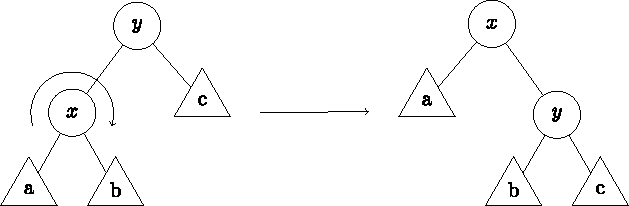
\includegraphics{imagens/zig.pdf}
    \label{fig:zig}

\caption{Passo splay zig onde $x$ é nó esquerdo da raiz.}
\end{figure}

%Esse passo splay é chamado de passo splay simples enquanto que os demais são passos splay duplos.

\begin{comment}
\begin{programruledcaption}{Função splay.\label{prog:abb-gulosa}}
    \noindent\textbf{Entrada}: Recebe um vértice $x$ de uma ABB \\
    \textbf{Saída}: ABB com as chaves 1 a $n$ com respeito ao vetor $e$.
    \vspace{-0.5\baselineskip}
    \begin{lstlisting}[
        language={[brazilian]pseudocode},
        style=pseudocode,
        style=wider,
        functions={},
        specialidentifiers={},
        escapeinside={(*@}{@*)},
    ]
    (*@\bfseries\scshape{Função}@*) splay(x)
        y := x.pai
        se y == NULL: // x é raiz
            (*@\textbf{retorne}@*)
        se y.pai == NULL: // x é filho da raiz
            se y.esq = x:
                (*@\textbf{então}@*) rotação_direita(x) // caso zig
                (*@\textbf{senão}@*) rotação_esquerda(x) // caso zag
        se y.esq == x e y.pai.esq == y // caso zig-zig
            (*@\textbf{então}@*) rotação_direita(x)
            (*@\textbf{senão}@*) rotação_esquerda(x)
        se y.esq == x e y.pai.dir == y // caso zig-zag
            (*@\textbf{então}@*) rotação_direita(x)
            (*@\textbf{senão}@*) rotação_esquerda(x)
        se y.dir == x e y.pai.dir == y // caso zag-zag
            (*@\textbf{então}@*) rotação_direita(x)
            (*@\textbf{senão}@*) rotação_esquerda(x)
        se y.dir == x e y.pai.esq == y // caso zag-zig
            (*@\textbf{então}@*) rotação_direita(x)
            (*@\textbf{senão}@*) rotação_esquerda(x)
    devolva abb
    \end{lstlisting}
    \vspace{-0.5\baselineskip}
\end{programruledcaption}
\end{comment}

Em algumas estruturas são definidas rotações direitas e esquerdas. %Seguiremos o modelo de computação adotado. 
A operação primitiva de rotação do modelo de computação adotado rotaciona o nó corrente com seu pai. Veja o Programa~\ref{prog:rotação}, que consome $\Oh(1)$. Essencialmente rotações para a direita e esquerda são rotações de um nó com um de seus filhos que precisa ser definido enquanto que rotações de um nó com seu pai é uma operação bem definida.

\begin{programruledcaption}{Função de rotação.\label{prog:rotação}}
    \noindent\textbf{Entrada}: Recebe um vértice $x$ de uma ABB que possui um vértice pai.\\
    \textbf{Saída}: Executa uma rotação de $x$ com seu pai. 
    \vspace{-0.5\baselineskip}
    \begin{lstlisting}[
        language={[brazilian]pseudocode},
        style=pseudocode,
        style=wider,
        functions={},
        specialidentifiers={},
        escapeinside={(*@}{@*)},
    ]
    (*@\bfseries\scshape{Função}@*) rotação_com_pai(x)
        y := x.pai
        z := y.pai
        se x = y.esq
            (*@\textbf{então}@*) y.esq := x.dir
            (*@\hspace{1.09cm}@*)x.dir := y
            (*@\hspace{1.09cm}@*)se y.esq != NULL
                (*@\hspace{1.09cm}@*)(*@\textbf{então}@*) y.esq.pai := y
            (*@\textbf{senão}@*) y.dir := x.esq
            (*@\hspace{1.08cm}@*)x.esq := y
            (*@\hspace{1.09cm}@*)se y.dir != NULL
                (*@\hspace{1.09cm}@*)(*@\textbf{então}@*) y.dir.pai := y
        x.pai := z
        y.pai := x
        se z != NULL
            se z.esq = y
                (*@\textbf{então}@*) z.esq := x
                (*@\textbf{senão}@*) z.dir := x

    \end{lstlisting}
    \vspace{-0.5\baselineskip}
\end{programruledcaption}

A seguir veja o código da operação splay no Programa~\ref{prog:splay} que se utiliza das rotações dadas no Programa~\ref{prog:rotação}. Além disso, a Figura~\ref{fig:fullsplay} ilustra a execução de uma operação splay onde há um passo splay zag-zag, um passo splay zig-zag e por fim um passo splay zig.

\begin{programruledcaption}{Função splay.\label{prog:splay}}
    \noindent\textbf{Entrada}: Recebe um vértice $x$ de uma ABB.\\
    \textbf{Saída}: Reestrutura a ABB com passos splay até $x$ ser raiz. 
    \vspace{-0.5\baselineskip}
    \begin{lstlisting}[
        language={[brazilian]pseudocode},
        style=pseudocode,
        style=wider,
        functions={},
        specialidentifiers={},
        escapeinside={(*@}{@*)},
    ]
    (*@\bfseries\scshape{Função}@*) splay(x)
        y := x.pai
        se y = NULL (*@ \hfill @*) // x é raiz
            (*@\textbf{retorne}@*)
        se y.pai = NULL (*@ \hfill @*) // zig/zag
            (*@\textbf{então}@*) rotação_com_pai(x)
        (*@\textbf{senão}@*) se y.esq = x e y.pai.esq = y ou y.dir = x e y.pai.dir = y (*@ \hfill @*) // zig-zig/zag-zag
            (*@\textbf{então}@*) rotação_com_pai(y)
            (*@\hspace{1.045cm}@*)rotação_com_pai(x)
        (*@\textbf{senão}@*) rotação_com_pai(x) (*@ \hfill @*) // zig-zag/zag-zig
            (*@\hspace{0.4cm}@*)rotação_com_pai(x)
        splay(x)
    \end{lstlisting}
    \vspace{-0.5\baselineskip}
\end{programruledcaption}

\begin{figure}
    \includegraphics[scale=0.77]{imagens/fullsplay2.pdf}
    \caption{Execução da operação splay após acesso à chave 4.}
\label{fig:fullsplay}
\end{figure}

Uma série de operações podem ser implementadas nessas estruturas como inserção, remoção, busca, junção e divisão. Todas essas operações chamam a operação splay no nó mais profundo visitado durante sua execução. É essencial entender que ao final de cada acesso, o nó com a chave acessada será levado para a raiz pela operação splay. O código da busca em árvores splay pode ser visto no Programa~\ref{prog:busca}.

No escopo desse trabalho só são consideradas buscas bem-sucedidas, porém com poucas modificações nos códigos, é possível tratar buscas mal-sucedidas. A diferença é que o nó mais profundo visitado não será o nó com chave buscada, então o nó que a rotina splay levará para a raiz é uma das folhas que possui chave vizinha à chave buscada. O mesmo acontece para remoções mal-sucedidas que também não são consideradas nesse texto.

\begin{programruledcaption}{Função de busca em árvores splay.\label{prog:busca}}
    \noindent\textbf{Entrada}: Recebe um inteiro $z$ no intervalo $[1,n]$ e um nó $x$ de uma árvore splay.\\
    \textbf{Saída}: Acessa o nó com chave $z$ e chama a rotina splay nele.
    \vspace{-0.5\baselineskip}
    \begin{lstlisting}[
        language={[brazilian]pseudocode},
        style=pseudocode,
        style=wider,
        functions={},
        specialidentifiers={},
        escapeinside={(*@}{@*)},
    ]
    (*@\bfseries\scshape{Função}@*) busca(z, x)
        se x.val = z
            (*@\textbf{então}@*) splay(x)
            (*@\textbf{retorne}@*)
        se x.val > z
            (*@\textbf{então}@*) busca(z, x.esq)
            (*@\textbf{senão}@*) busca(z, x.dir)
        
    \end{lstlisting}
    \vspace{-0.5\baselineskip}
\end{programruledcaption}

\section{Análise da operação splay}

Definimos o custo da operação splay como o número de rotações realizadas durante sua execução. Caso nenhuma rotação seja realizada, definimos o custo dessa operação como 1. 
%ONDE EU USEI QUE A ROTAÇÃO TEM CUSTO 1?

Faremos uma análise amortizada da estrutura pelo método do potencial. Seja $S$ a árvore splay sendo analisada. Definimos $s^{i}(x)$ como o tamanho da subárvore enraizada no nó $x$ de $S$ depois do passo splay $i$ de uma rotina splay. Definimos o potencial local do nó $x$ logo depois do passo splay $i$ como $r^{i}(x) = \lg(s^{i}(x))$. Por fim, definimos $c$ como o custo real de uma operação splay, \( \hat{c}\) como o custo amortizado de uma operação splay e $\Phi^{i}(S)$ como o potencial da árvore $S$ depois do passo splay $i$, que é a somatória do potencial local de todos os nós de $S$ nesse instante de tempo.

Para deduzir o custo amortizado de uma operação splay($x$), vamos calcular o custo amortizado de cada passo splay realizado dentro da operação splay. Note que todos esses passos envolvem o nó $x$.

\begin{lemma}
    Se o $j$-ésimo passo splay de uma rotina splay é um passo splay simples, então seu custo amortizado é menor que $3(r^{j}(x) - r^{j-1}(x)) + 1$.
    %O custo amortizado de um passo splay simples no nó $x$ é $< 3(r^{j}(x) - r^{j-1}(x)) + 1$, onde esse passo splay é o $j$-ésimo de uma rotina splay.
\end{lemma}

\begin{proof}
    Denotemos por $y$ o nó pai de $x$ que é a raiz da árvore splay logo antes do último passo splay. Se o passo splay simples é um passo zig, então $c = 1$ e
    \begin{align*}
        \hat{c} &= c + \Delta \Phi,\\
        &= 1 + r^{j}(x) + r^{j}(y) - r^{j-1}(x) - r^{j-1}(y), \quad & \text{}\\
        &< 1 + r^{j}(x) - r^{j-1}(x) \quad & \text{pois $r^{j-1}(y) > r^{j}(y)$},\\
        &< 1 + 3(r^{j}(x) - r^{j-1}(x)) \quad & \text{pois $r^{j}(x) > r^{j-1}(x)$}.\\
    \end{align*}
    O mesmo vale simetricamente para o caso zag.
\end{proof}

\newpage

\begin{lemma}
    Se o $j$-ésimo passo splay de uma rotina splay é um passo splay duplo, então seu custo amortizado é menor que $3(r^{j}(x) - r^{j-1}(x))$.
    %O custo amortizado de qualquer passo splay duplo no nó $x$ é $< 3(r^{j}(x) - r^{j-1}(x)) + 1$, onde esse passo splay é o $j$-ésimo de uma rotina splay.
\end{lemma}

\begin{proof}
    Para os próximos resultados será essencial entender uma propriedade da função logaritmo. A função logaritmo é côncava, ou seja, $\frac{\lg(a) + \lg(b)}{2} \leq \lg(\frac{a+b}{2})$. Isso pode ser evidenciado pela Figura~\ref{fig:log}.

    \begin{figure}
        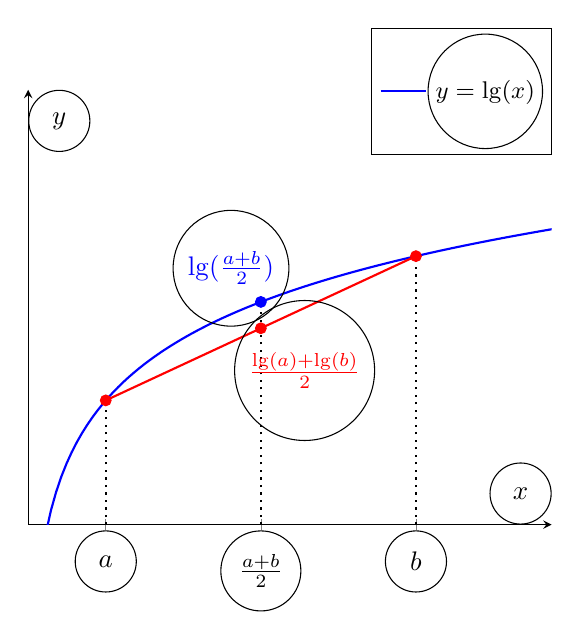
\begin{tikzpicture}[scale=0.97]
            \begin{axis}[
                axis lines = middle,
                xmin=0, xmax=27,
                ymin=0, ymax=7,
                xtick={4,12,20},
                xticklabels={$a$,$\frac{a+b}{2}$,$b$},
                ytick=\empty,
                xlabel = {$x$}, % Nome do eixo x
                ylabel = {$y$},
                legend style={
                    at={(1,0.85)},  % Move a legenda mais para baixo
                    anchor=south east,
                    font=\small   % Reduz o tamanho da fonte da legenda
                }
            ] % Função y = log2(x)
                \addplot[blue, thick, domain=0.1:40, samples=150] {log2(x)};
                
                % Pontos
                \addplot[only marks, red] coordinates {(4,2)}; % Ponto A
                \addplot[only marks, red] coordinates {(20, 4.3219281)}; % Ponto B
                \addplot[only marks, blue] coordinates {(12,3.5849625)}; % Ponto C
                \addplot[only marks, red] coordinates {(12,3.16096405)}; % Ponto D
        
                % Reta entre A e B
                \addplot[red, thick] coordinates {(4,2) (20, 4.3219281)};
                
                % Linhas pontilhadas
                \draw[thick, dotted] (axis cs:4,0) -- (axis cs:4,2);   % Linha pontilhada de A
                \draw[thick, dotted] (axis cs:20,0) -- (axis cs:20, 4.3219281);   % Linha pontilhada de B
                \draw[thick, dotted] (axis cs:12,0) -- (axis cs:12, 3.5849625);
                
                % Nomes dos pontos
                \node at (axis cs:12, 3.5849625) [anchor=south east, text = blue, xshift=0.15cm, yshift=-0.1cm] {$\lg(\frac{a+b}{2})$};  % Nome do ponto C
                \node at (axis cs:12, 3.16096405) [anchor=north west, text=red, xshift=-0.08cm, yshift=0.1cm] {$\frac{\lg(a) + \lg(b)}{2}$};  % Nome do ponto D
                
                % Legenda
                \addlegendentry{$y = \lg(x)$} % Legenda para a função
            \end{axis}
        \end{tikzpicture}
    \caption{Na imagem estão destacados pontos $a$ e $b$ arbitrários na função. Como a função é côncava, o ponto com $y = \frac{\lg(a) + \lg(b)}{2}$ nunca estará acima do ponto com $y = \lg(\frac{a+b}{2})$.}
    \label{fig:log}
    \end{figure}

    Denotemos por $y$ o nó pai de $x$ antes do passo splay analisado e por $z$ o avô de $x$ no mesmo instante. Se o passo splay duplo é um passo zig-zig, então $c = 2$ e
    \begin{align*}
        %\hat{c} &= c + \Delta \Phi, & \hspace*{-1.2cm} \text{amortizado = custo + diferença de potencial}, \\
        \hat{c} &= c + \Delta \Phi,\\
        &= 2 + r^{j}(x) + r^{j}(y) + r^{j}(z) - r^{j-1}(x) - r^{j-1}(y) - r^{j-1}(z), \quad & \text{}\\
        &= 2 + r^{j}(y) + r^{j}(z) - r^{j-1}(x) - r^{j-1}(y) \quad & \text{pois $r^{j}(x) = r^{j-1}(z)$},\\
        &< 2 + r^{j}(y) + r^{j}(z) - 2r^{j-1}(x) \quad & \text{pois $r^{j-1}(y) > r^{j-1}(x)$}, \\
        &< 2 + r^{j}(x) + r^{j}(z) - 2r^{j-1}(x) \quad & \text{pois $r^{j}(x) > r^{j}(y)$}.
    \end{align*}
    Por conta da concavidade da função $\lg$ vista acima, temos que:
    \begin{align*}
        %\hat{c} &= c + \Delta \Phi, & \hspace*{-1.2cm} \text{amortizado = custo + diferença de potencial}, \\
        r^{j-1}(x) + r^{j}(z) &= \lg(s^{j-1}(x)) + \lg(s^{j}(z)), \quad & \text{}\\
        &= 2 \cdot \frac{\lg(s^{j-1}(x)) + \lg(s^{j}(z))}{2}, \quad & \text{} \\
        &\leq 2 \lg(\frac{s^{j-1}(x) + s^{j}(z)}{2}) \quad & \text{concavidade de $\lg$}, \\
        &< 2 \lg(\frac{s^{j}(x)}{2}) \quad & \text{pois $s^{j}(x) > s^{j-1}(x) + s^{j}(z)$}, \\
        &= 2 (\lg(s^{j}(x)) - \lg(2)),\\
        &= 2 (r^{j}(x) - 1).
    \end{align*}
    Assim, retornando ao problema original,
    \begin{align*}
        \hat{c} &< 2 + r^{j}(x) + r^{j}(z) - 2r^{j-1}(x), \\
        &< 2 + r^{j}(x) +  2 (r^{j}(x) - 1) - r^{j-1}(x) - 2r^{j-1}(x), \\
        &= 3(r^{j}(x) - r^{j-1}(x)). \\
    \end{align*}
    O mesmo vale para o caso zag-zag por simetria. \\ \\ Se o passo splay duplo é um passo zig-zag, então $c = 2$ e
    \begin{align*}
        %\hat{c} &= c + \Delta \Phi, & \hspace*{-1.2cm} \text{amortizado = custo + diferença de potencial}, \\
        \hat{c} &= c + \Delta \Phi,\\
        &= 2 + r^{j}(x) + r^{j}(y) + r^{j}(z) - r^{j-1}(x) - r^{j-1}(y) - r^{j-1}(z), \quad & \text{}\\
        &= 2 + r^{j}(y) + r^{j}(z) - r^{j-1}(x) - r^{j-1}(y) \quad & \text{pois $r^{j}(x) = r^{j-1}(z)$},\\
        &< 2 + r^{j}(y) + r^{j}(z) - 2r^{j-1}(x) \quad & \text{pois $r^{j-1}(x) < r^{j-1}(y)$},\\
        &< 2 + r^{j}(x) - 2r^{j-1}(x) \quad & \text{pois $r^{j}(y) + r^{j}(z) < r^{j}(x)$},\\
        &< 3(r^{j}(x) - r^{j-1}(x)). \\
    \end{align*}
    O mesmo vale para o caso zag-zig por simetria.
\end{proof}

\begin{theorem}
    O custo amortizado da operação splay é $\Oh(\lg n)$.
\end{theorem}

\begin{proof}
    Caso a operação splay não faça rotações, o custo é 1 e a delimitação é imediata. Caso contrário, o custo amortizado da operação splay no nó $x$ é a soma dos custos amortizados dos passos splay realizados durante a operação.

    Denotemos por $\hat{c}_{\textit{splay}}$ o custo amortizado da operação splay e por $\hat{c}_{i}$ o custo amortizado do $i$-ésimo passo splay realizado durante o Splay($x$). Denotemos por $t$ o número de passos splay realizados por essa operação. Então
    \begin{align*}
        \hat{c}_{\textit{splay}} &= \sum_{i = 1}^{t} \hat{c}_{i}, \\
        &< \sum_{i = 1}^{t} {3(r^{i}(x) - r^{i-1}(x)) + 1}, \\
        &= 3(r^{t}(x) - r^{0}(x)) + 1, \\ 
        &\leq 3(r^{t}(x)) + 1 \quad & \text{pois $r^{0}(x) \geq 0$}, \\  
        &= 3\lg n + 1 \quad & \text{pois $r^{t}(x) = \lg(n)$}, \\ 
        &= \Oh(\lg n).
    \end{align*}
\end{proof}
\newpage

\begin{theorem}
    Se $m = \Omega(n)$, então uma sequência de $m$ acessos em uma árvore splay possui custo $\Oh(m \lg n)$.
\end{theorem}

\begin{proof}
Note que $\Phi^{0}(S)$ é a soma do potencial local de todos os nós de $S$ durante esse instante de tempo. Assim, sabemos que 
\begin{align*}
    \Phi^{0}(S) &= \sum_{x = 1}^{n}r^{0}(x) \quad & \text{pela definição de $\Phi^{0}(S)$},\\
    &= \sum_{x = 1}^{n}\lg(s^{0}(x)) \quad & \text{pela definição de $r^{0}(x)$},\\
    &\leq \sum_{x = 1}^{n}\lg n \quad & \text{pois $s^{0}(x) \leq n$},\\
    &= n\lg n.\\
\end{align*}

Essa propriedade será utilizada abaixo. Considere uma sequência de $m$ acessos em uma árvore splay $S$. Então
\begin{align*}
    \sum_{i = 1}^{m} c_i &= \sum_{i = 1}^{m} (\hat{c}_i + \Phi^{i-1}(S) - \Phi^{i}(S)),\\
    &= \sum_{i = 1}^{m} \hat{c}_i + \Phi^{0}(S) - \Phi^{m}(S),\\
    &\leq \sum_{i = 1}^{m} \hat{c}_i + \Phi^{0}(S) \quad & \text{pois $\Phi^{m}(S) \geq 0$},\\
    &\leq m(3\lg n + 1) + n\lg n \quad & \text{pois $\Phi^{0}(S) \leq n\lg n$},\\
    &= (3m + n)(\lg n) + m, \\
    &= \Oh(m \lg n) \quad & \text{se $m = \Omega(n)$}.
\end{align*}
\end{proof}

\section{Conjectura da Otimalidade Dinâmica}

Uma ABB online é \textit{dinamicamente ótima} se, para todas as sequências $X$ de acessos, seu algoritmo de busca tem custo $\Oh(\text{\OPT}(X))$. De maneira mais geral, uma ABB online é \textit{$c$-competitiva} se executa todas as buscas para sequências $X$ suficientemente longas com custo no máximo $c$\,\OPT$(X)$.

Sleator e Tarjan \cite{selfadjustingbst} conjecturaram que a árvore splay é dinamicamente ótima. Essa conjectura é conhecida por Conjectura da Otimalidade Dinâmica. Os cientistas nas últimas décadas vêm buscando provar propriedades que \OPT$(X)$ e as árvores splay possuem em comum. Uma série de características foram detectadas e o ramo de pesquisa se mantém ativo. É impressionante que em uma área tão amplamente pesquisada como a área de estrutura de dados, essa conjectura continue em aberto, intrigando cientistas pela sua dificuldade.

Pouco se sabe sobre o valor de \OPT$(X)$ para uma sequência $X$ de acessos. No próximo capítulo abordaremos uma visão geométrica de buscas e em seguida buscaremos entender quais são as características de \OPT$(X)$ dentro dessa abordagem. 